% File 	: proj5.tex
% Author	: Matus Liscinsky
% Login	: xlisci02
% Email	: xlisci02@stud.fit.vutbr.cz
% Date	: 12.05.2017
% About	: Projekt č.5 do predmetu ITY

\documentclass{beamer}
 
\usepackage[czech]{babel}
\usepackage[utf8]{inputenc}
\usepackage{graphics}
\usepackage{sidecap}

\usepackage{amsmath}
\usepackage[T1]{fontenc}
\usepackage{lmodern}
\usepackage{amssymb}

%Titulna strana
\usecolortheme{whale}
\title{Möbiov list}
\author{Matúš Liščinský \\ 
\small{\url{xlisci02@stud.fit.vutbr.cz}}}
\institute{Vysoké učení technické v~Brně \\
Fakulta informačních technologií}

\date{2017}
 
\begin{document}

\frame{\titlepage}
 
\begin{frame}
\frametitle{Úvod}
\begin{itemize}
\item Möbiova páska, Simonyho prstenec
\item 1858 -- August Ferdinand Möbius, Johann Benedikt Listing
\item Plocha, ktorá má len jednu stranu a~jednu hranu
\item Ukážka deformácie dvojrozmernej plochy do tretieho rozmeru
\end{itemize}
\centering
\vspace*{0.5cm}
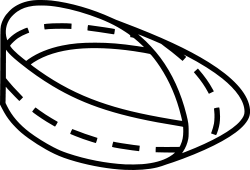
\includegraphics[width=4cm]{paska.png}
\end{frame}

\begin{frame}
\frametitle{Matematický popis}
\begin{itemize}
\item Jednotkovú Möbiovu pásku možno jednoducho popísať parametrickými rovnicami:
\begin{itemize}
\item $x = \cos(\alpha) + p \cos(\frac{\alpha}{2}) \cos(\alpha) $
\item $y = \sin(\alpha) + p \cos(\frac{\alpha}{2}) \sin(\alpha) $
\item $z = p \sin(\frac{\alpha}{2}) $
\end{itemize}
\item[] kde $\alpha$ a $p$ sú parametre pre ktoré platí:
\begin{itemize}
\item $0 \leq \alpha \leq 2\pi$
\item $p_{min} \leq p \leq p_{max}$
\end{itemize}
\item Hodnoty $p_{min}$ a $p_{max}$ určujú šírku pásky z~intervalu (-1,1)
\end{itemize}

\end{frame} 

\begin{frame}
\frametitle{Vytvorenie Möbiovho listu}
\centering
\begin{itemize}
\item Pásik papiera
\item Jeden koniec priečne pretočíme 
\item Zlepíme s~druhým koncom  
\end{itemize}
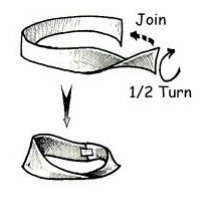
\includegraphics[width=5cm]{priprava.png}
\end{frame} 

\begin{frame}
\frametitle{Ďalšie efekty}
\centering
\begin{itemize}
\item Čo sa stane ak ? 
\bigskip
\begin{itemize}
\item Pásku rozstrihneme v~strede ? 
\begin{itemize}
\item[]
\medskip
\end{itemize}
\item Pásku rozstrihneme po okraji ? 
\begin{itemize}
\item[]
\medskip
\end{itemize}
\item Budeme chcieť namaľovať každú stranu inou farbou? 
\begin{itemize}
\item[]
\medskip
\end{itemize}
\end{itemize}
\end{itemize}
\end{frame} 

\begin{frame}
\frametitle{Ďalšie efekty}
\centering
\begin{itemize}
\item Čo sa stane ak ? 
\bigskip
\begin{itemize}
\item Pásku rozstrihneme v~strede ? 
\begin{itemize}
\item  Vznikne jeden dlhý, niekoľkokrát pretočený pruh
\medskip
\end{itemize}
\item Pásku rozstrihneme po okraji ? 
\begin{itemize}
\item []
\medskip
\end{itemize}
\item Budeme chcieť namaľovať každú stranu inou farbou? 
\begin{itemize}
\item []
\medskip
\end{itemize}
\end{itemize}
\end{itemize}
\end{frame} 

\begin{frame}
\frametitle{Ďalšie efekty}
\centering
\begin{itemize}
\item Čo sa stane ak ? 
\bigskip
\begin{itemize}
\item Pásku rozstrihneme v~strede ? 
\begin{itemize}
\item  Vznikne jeden dlhý, niekoľkokrát pretočený pruh
\medskip
\end{itemize}
\item Pásku rozstrihneme po okraji ? 
\begin{itemize}
\item Vzniknú dva do seba vpletené pruhy
\medskip
\end{itemize}
\item Budeme chcieť namaľovať každú stranu inou farbou? 
\begin{itemize}
\item []
\medskip
\end{itemize}
\end{itemize}
\end{itemize}
\end{frame} 

\begin{frame}
\frametitle{Ďalšie efekty}
\centering
\begin{itemize}
\item Čo sa stane ak ? 
\bigskip
\begin{itemize}
\item Pásku rozstrihneme v~strede ? 
\begin{itemize}
\item  Vznikne jeden dlhý, niekoľkokrát pretočený pruh
\medskip
\end{itemize}
\item Pásku rozstrihneme po okraji ? 
\begin{itemize}
\item Vzniknú dva do seba vpletené pruhy
\medskip
\end{itemize}
\item Budeme chcieť namaľovať každú stranu inou farbou? 
\begin{itemize}
\item Páska obsahuje len jednu stranu
\end{itemize}
\end{itemize}
\end{itemize}
\end{frame} 


\begin{frame}
\frametitle{Zaujímavosti}
\title{Využitie}
\begin{itemize}
\item Využitie
\begin{itemize}
\item hnacie remene s~dlhšou životnosťou
\item dopravníkové pásy - nekonečná prehrávacia slučka (dvojnásobná dĺžka záznamu)
\end{itemize}
\end{itemize}

\begin{itemize}
\item{Ďalšie zaujímavé odkazy}
\begin{itemize}
\item \href{https://cs.wikipedia.org/wiki/Penrose\%C5\%AFv_troj\%C3\%BAheln\%C3\%ADk}{Penroseov trojuholník}
\item \href{https://cs.wikipedia.org/wiki/Kleinova_l\%C3\%A1hev}{Kleinova fľaša}
\end{itemize}
\end{itemize}
\end{frame} 

\begin{frame}
\frametitle{Zdroje}

\begin{itemize}
\item The Magical Möbius Strip \\
\url{http://www.maths.ed.ac.uk/~jcollins/MobiusInstructions.pdf}
\item Wikipedia \\
\url{https://sk.wikipedia.org/wiki/M\%C3\%B6biov_list}\\
\url{https://cs.wikipedia.org/wiki/M\%C3\%B6biova_p\%C3\%A1ska\#Matematick.C3.BD_popis}
\item Youtube -- Möbiova páska \\
\url{https://www.youtube.com/watch?v=YqCmu1ppKqQ}
\end{itemize}
\end{frame} 


\end{document}